\documentclass[10pt]{article}

\usepackage{fullpage}
\usepackage{graphicx}
\usepackage{graphics}
\usepackage{mdwlist}
\usepackage[top=2.5cm, bottom=2.5cm, left=2.5cm, right=2.5cm]{geometry}
\usepackage{kotex}

\setlength{\oddsidemargin}{0.0in}
\setlength{\evensidemargin}{0.0in}
\setlength{\textwidth}{6.5in}
\setlength{\headheight}{0.0in}
\setlength{\topmargin}{0.0in}
% \setlength{\textheight}{9.0in}
\setlength{\textheight}{9in}
\addtolength{\textheight}{-\topmargin}
\addtolength{\textheight}{-\headheight}
\addtolength{\textheight}{-\headsep}
\addtolength{\textheight}{-\footskip}

\begin{document}

\newcommand{\beq}{\begin{equation}}
\newcommand{\eeq}{\end{equation}}
\newcommand{\bit}{\begin{itemize*}}
\newcommand{\eit}{\end{itemize*}}
\newcommand{\goal}[1]{ {\noindent {$\Rightarrow$} \em {#1} } }
\newcommand{\hide}[1]{}
\newcommand{\comment}[1]{ {\footnotesize {#1} } }
\newtheorem{lemma}{Lemma}
\newtheorem{theorem}{Theorem}
\newtheorem{proof}{Proof}
\newtheorem{defn}{Definition}
\newtheorem{algo}{Algorithm}
\newtheorem{observation}{Observation}

\title{Online Tensor Analysis}

\author{ {\em Sangjun Son} \\
	    Computer Science and Engineering \\
	    Seoul National University\\
	    {\tt lucetre@snu.ac.kr}
	 \and
	 {\em U Kang} \\
	    Computer Science and Engineering \\
	    Seoul National University\\
	     {\tt ukang@snu.ac.kr}
        }


\maketitle
\begin{abstract}
    
In this paper, we propose fast and accurate online tensor decomposition method called {\em OnlineTensorAnalysis}, which performs splitting its tensor and create a new factorization when drastic data change detection.

\end{abstract}

\section{Introduction}
    \label{sec:intro}
    
Given a temporally growing tensor, how can we analyze it efficiently? Multi-dimensional arrays or tensors have been widely used to model real world data. Tensor decomposition plays an significant role in latent feature detection and prediction of unobservable entries. Each tensor can have different lengths of modes and tensors having their size consistent are called static, and the others are called dynamic tensors. Most of existing tensor analysis methods such as CP-ALS or HOSVD decompose static tensors with high fitness. However, applying static tensor decomposition methods to dynamic tensors is actually an inappropriate way in time and space efficiency.

For tensors dynamically growing in the temporal mode (e.g. sensor data on every point of the room), their factorization invokes lots of computations to update all the entries on time factor. Data stream produces numerous amounts of data incomes every second and it became more important to maintain each tensor factorization results. The contributions of this project are the following:
\bit
\item our proposed {\em OnlineTensorAnalysis} performs online tensor decomposition preserving accuracy without time dilation due to short data income intervals.
\item it is time scalable, being linear on the length of temporal mode. 
\item it automatically detects drastic data changes and creates starting points of decomposition for accuracy optimization.
\eit

\section{Preliminaries}
    \label{sec:prelim}
    \subsection{Preliminaries}
...
    
\newpage
\section{Proposed Method}
    \label{sec:proposed}
  	
We've developed our methods by extending the basic intuition of \ocp. Since dynamic tensor decomposition pursues shorter time factor updates, this results low accuracy factorization when real-time data incomes. To optimize the speed accuracy problem, we'd like to trigger static decomposition method, \cpals while dynamic method like \ocp is being done.

\begin{center}
	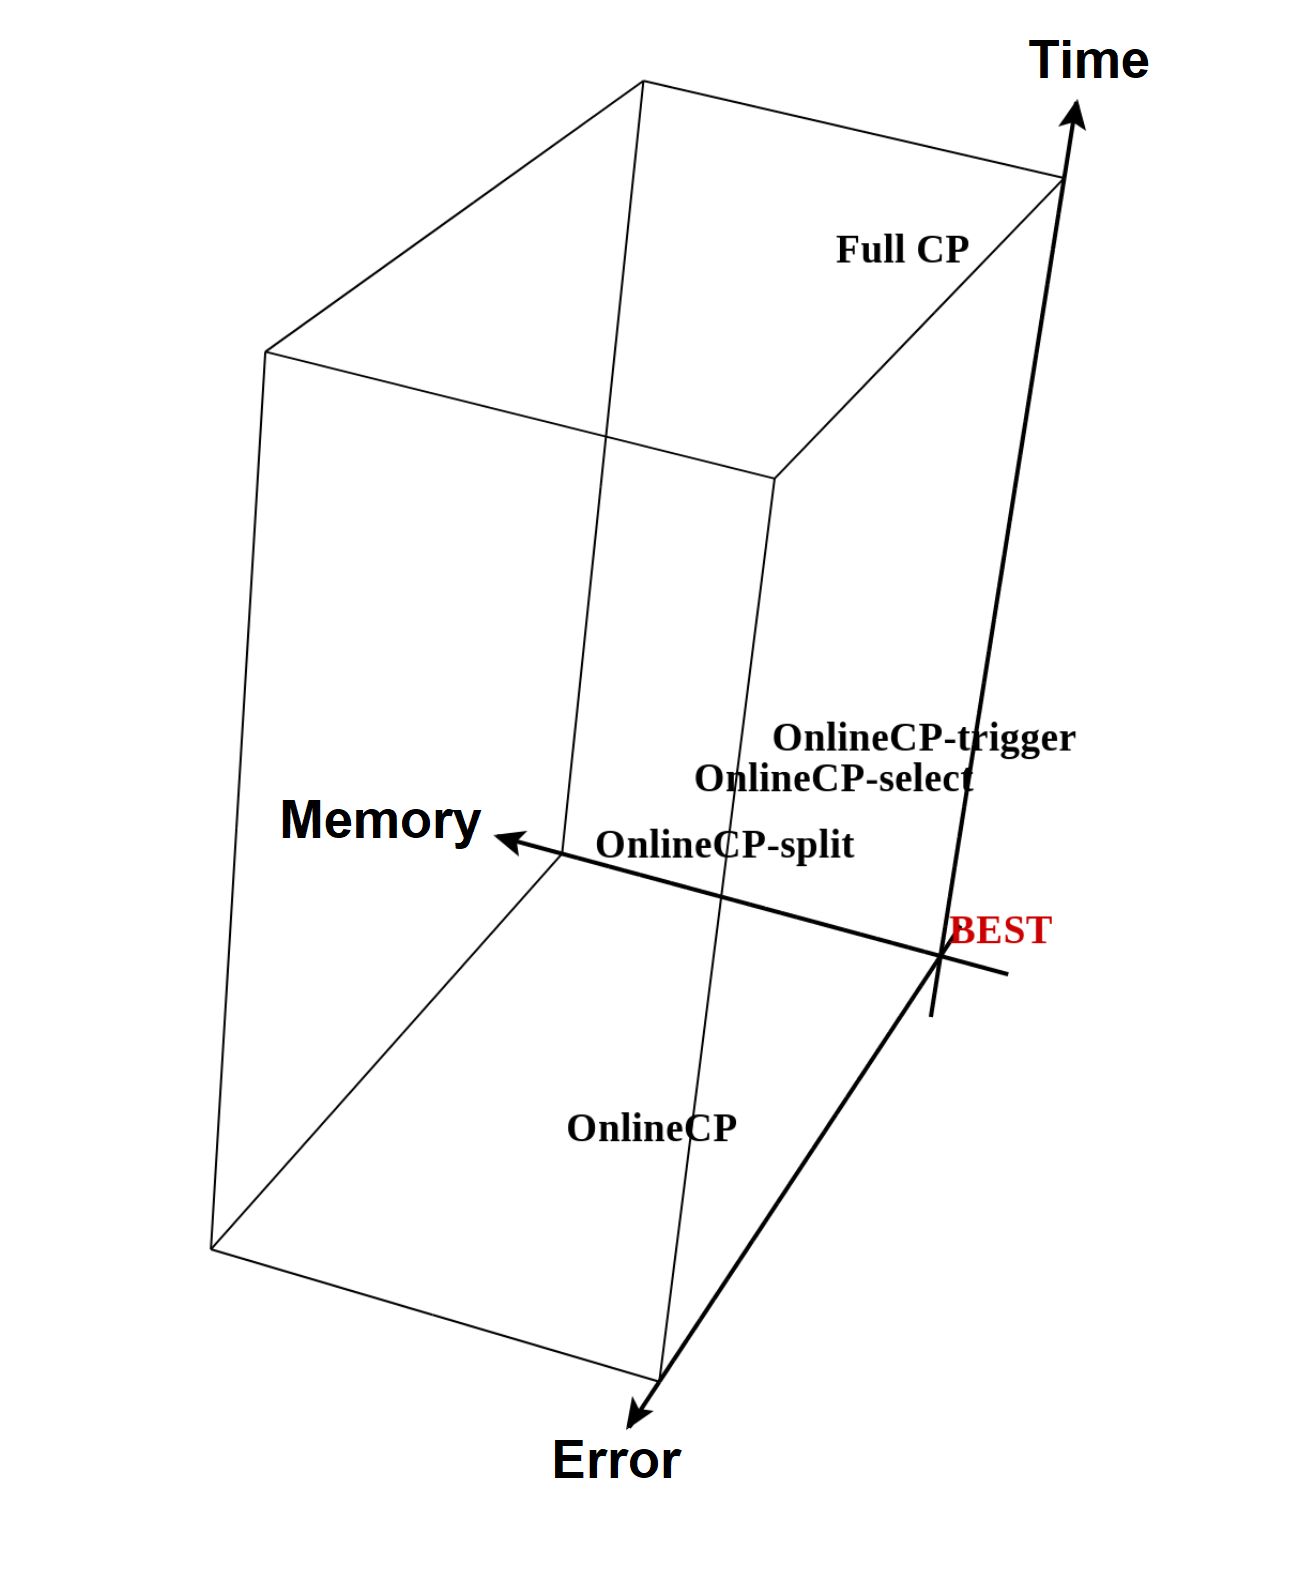
\includegraphics[width=0.49\textwidth]{FIG/method-comparison1.png}
	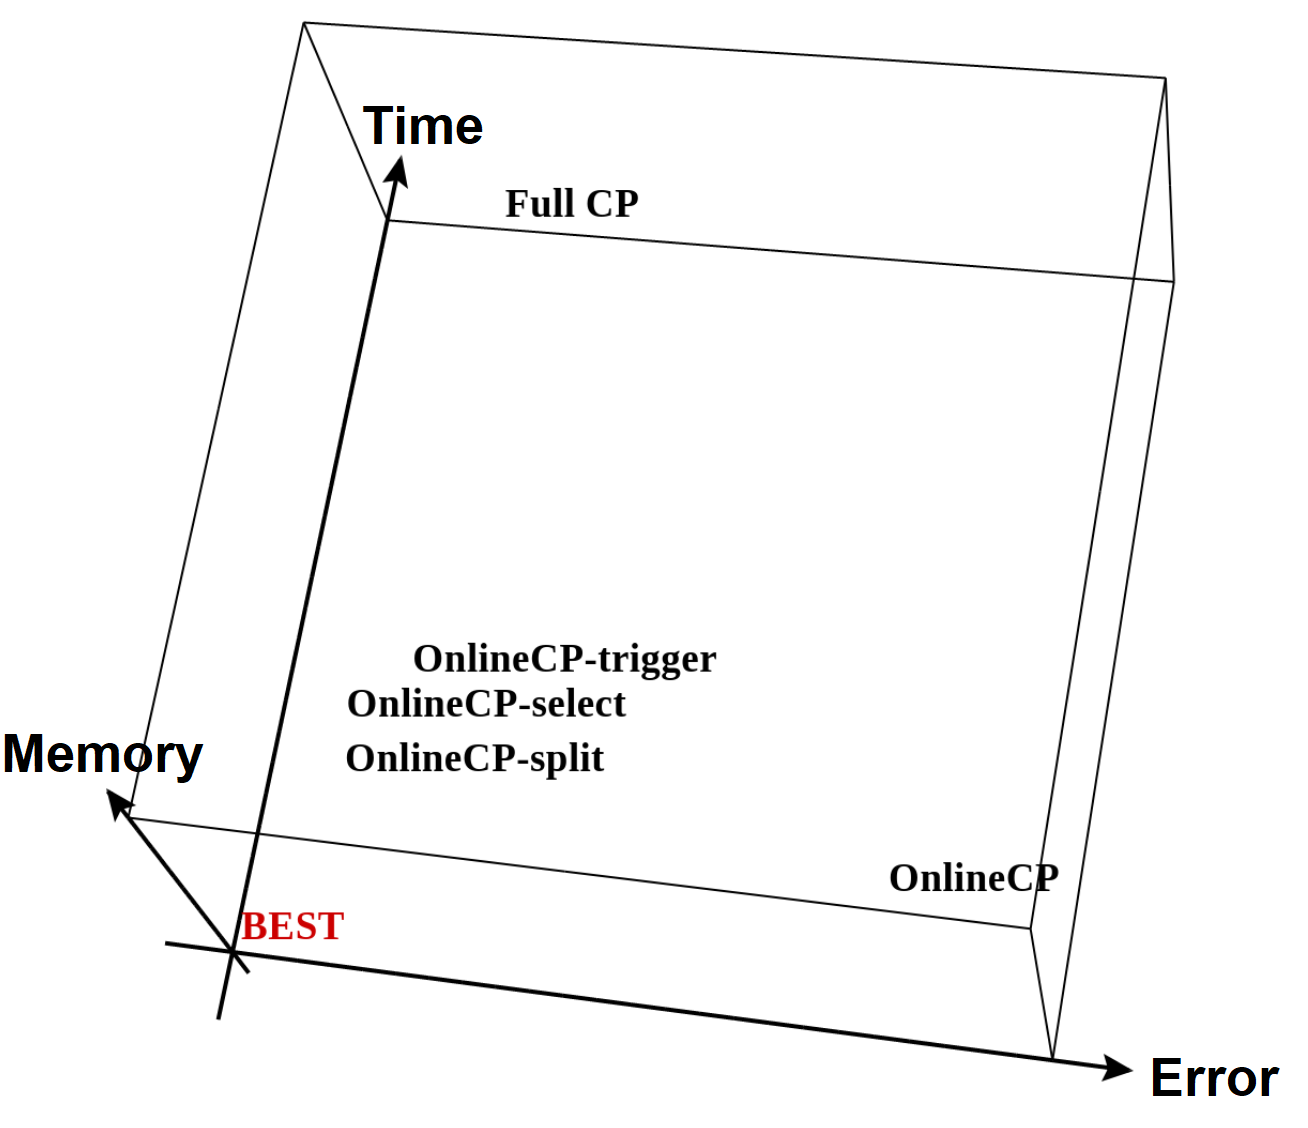
\includegraphics[width=0.49\textwidth]{FIG/method-comparison3.png}
\end{center}
\begin{center}
	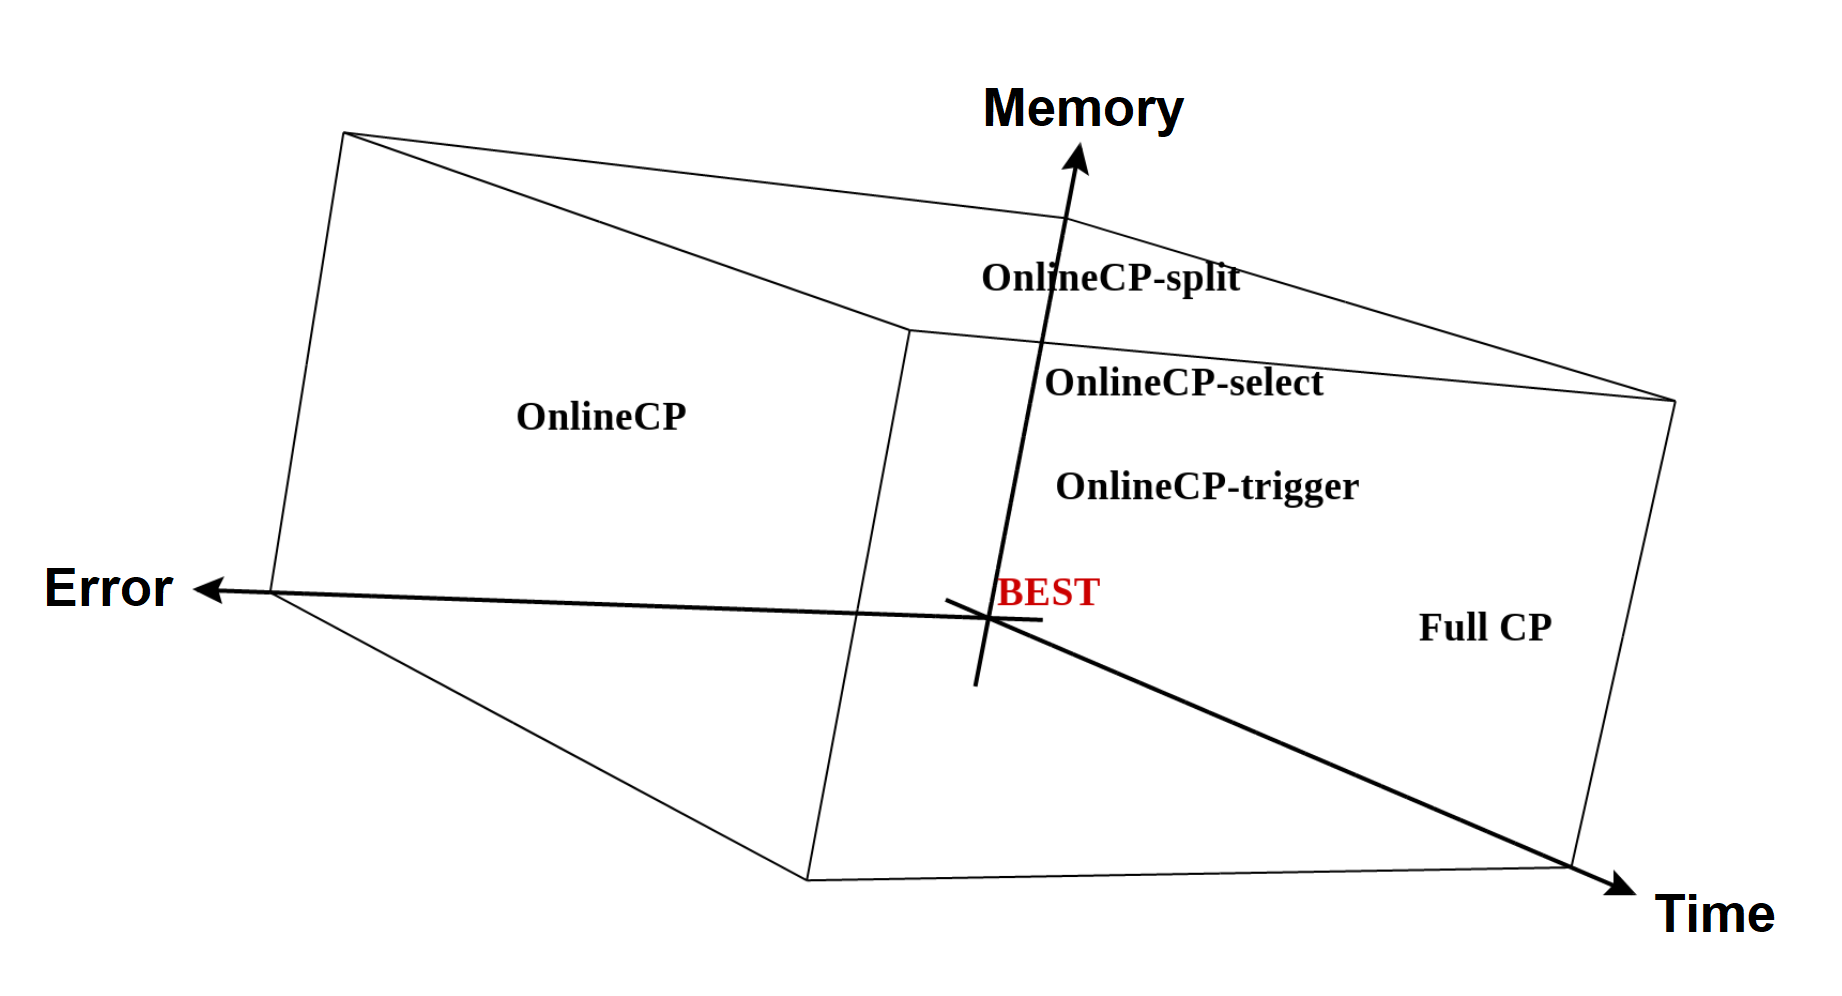
\includegraphics[width=1\textwidth]{FIG/method-comparison2.png}
\end{center}

\newpage
\subsection{\em OnlineCP-trigger}
\textbf{Detection Approach}: \cpals activates whole temporal factor updates and enables high accuracy decomposition. Drastic data can be detected by calculating image error norm and its ratio between neighboring time steps. The moment for triggering \cpals is when temporal ratio of error norm for incoming data exceeds threshold.

\begin{align*}
    threshold < \frac{\norm{\tilde{\chi}_{i+1}-\chi_{i+1}}}{\norm{\tilde{\chi}_{i}-\chi_{i}}}
\end{align*}

\begin{center}
	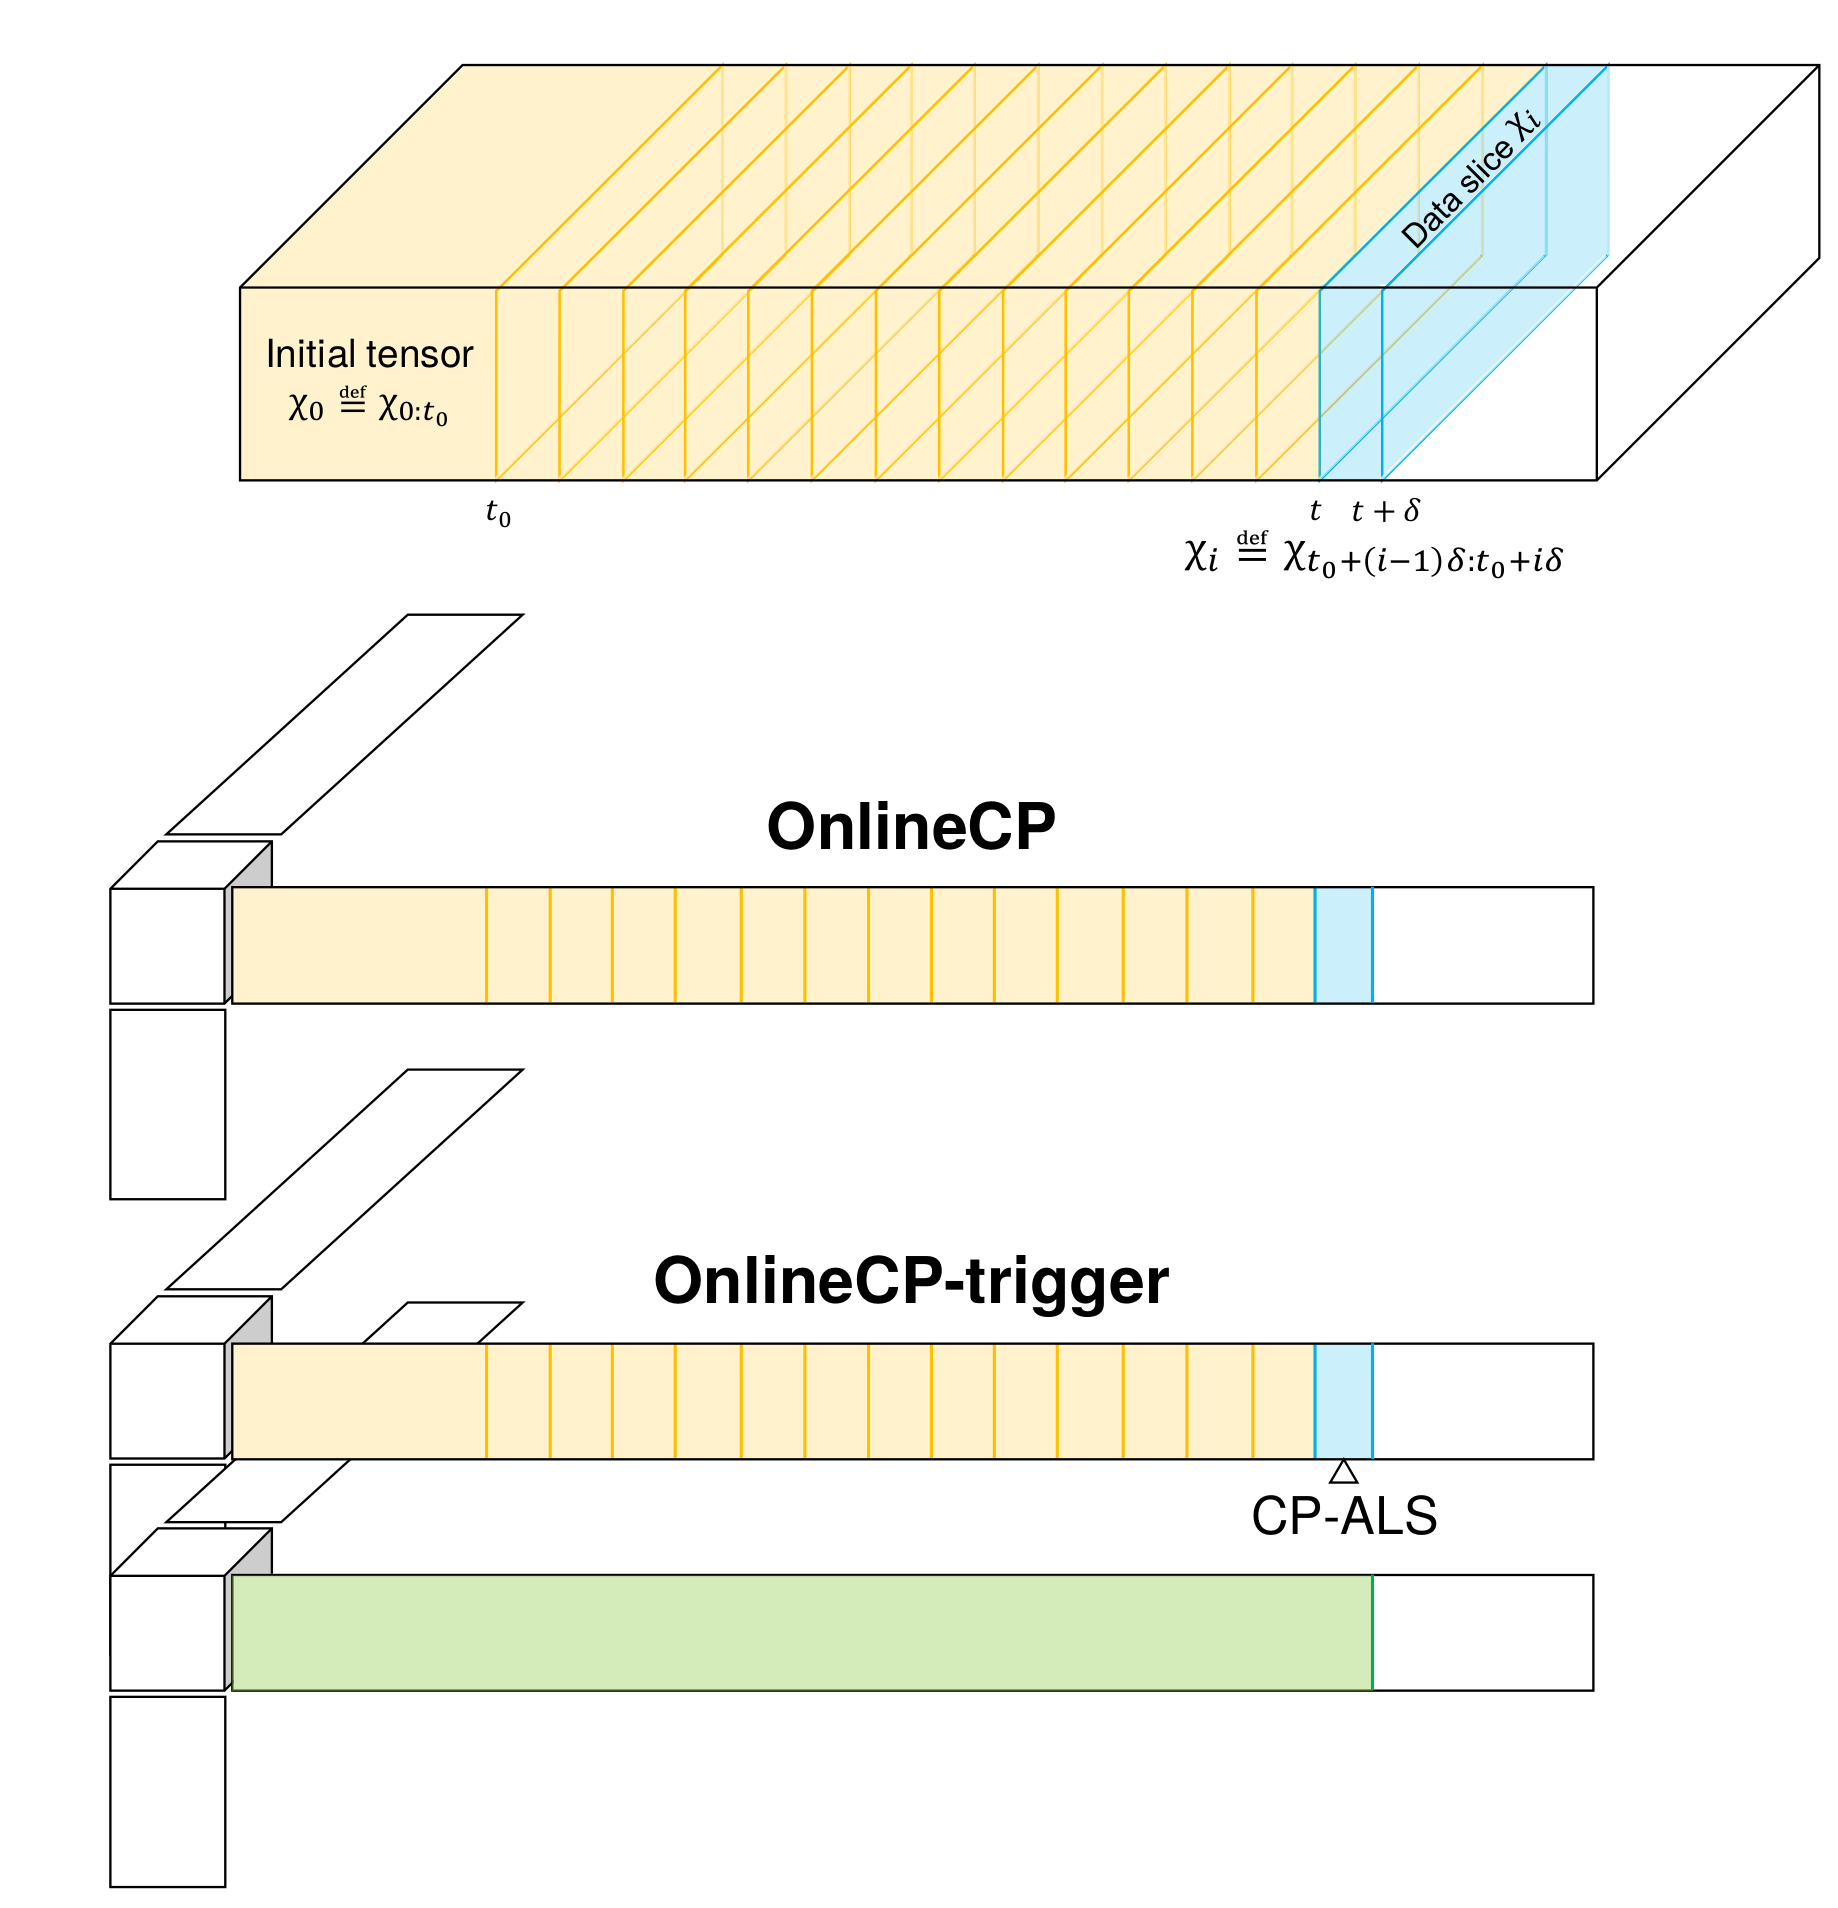
\includegraphics[width=0.85\textwidth]{FIG/OnlineCP-trigger.png}
\end{center}

\newpage
\subsection{\em OnlineCP-split}
\textbf{Split Approach}: trigger function in detection approach tells us sudden change in data. What if the incoming data may have a new theme unseen before? It implies that new decomposition starting point with tensor split is needed. In this approach, we'd like to apply the trigger function for splitting the tensor into serial tensors of different themes. (e.g. $A$, $B$, $C$, $D$)

\begin{center}
	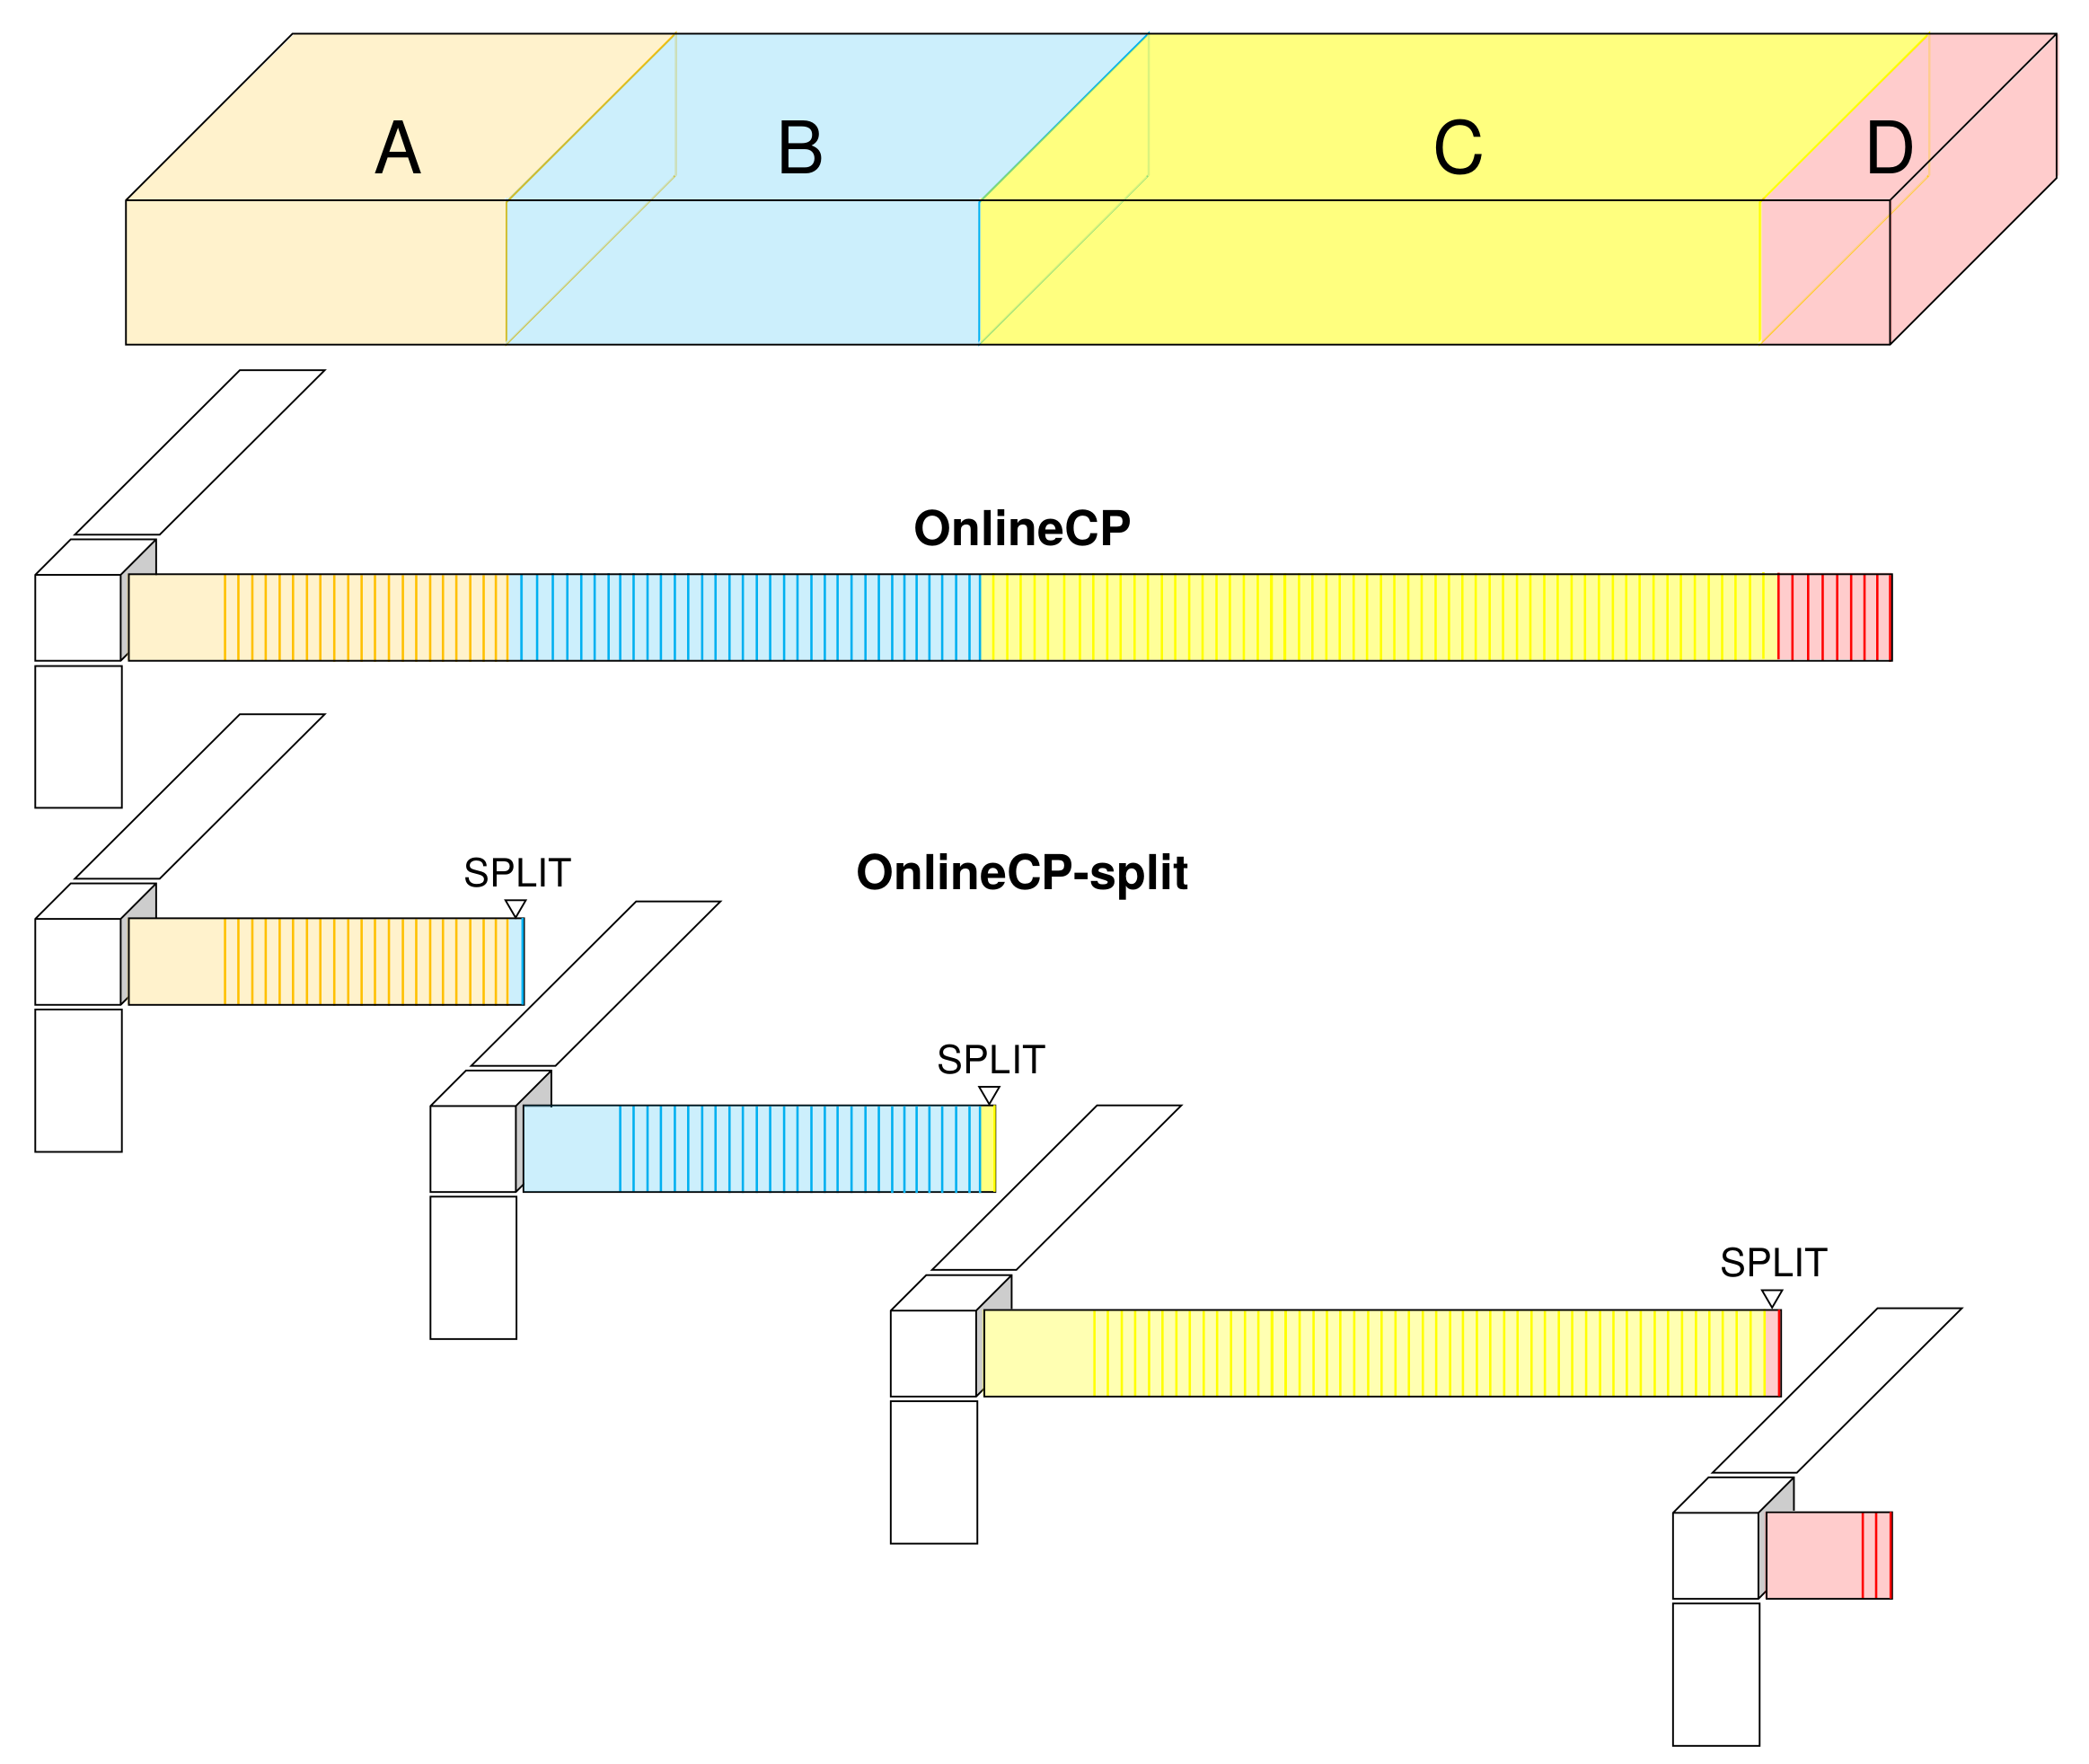
\includegraphics[width=0.9\textwidth]{FIG/OnlineCP-split.png}
\end{center}

\newpage
\subsection{\em OnlineCP-select}
\textbf{Selection Approach}: Similarly to split approach, trigger function now decides whether to split or to concatenate behind after one temporal factor update. It allows to store the tensor efficiently; group tensors with similar themes and split them otherwise. (e.g. $A$, $B$, $B'$, $C$)

\begin{center}
	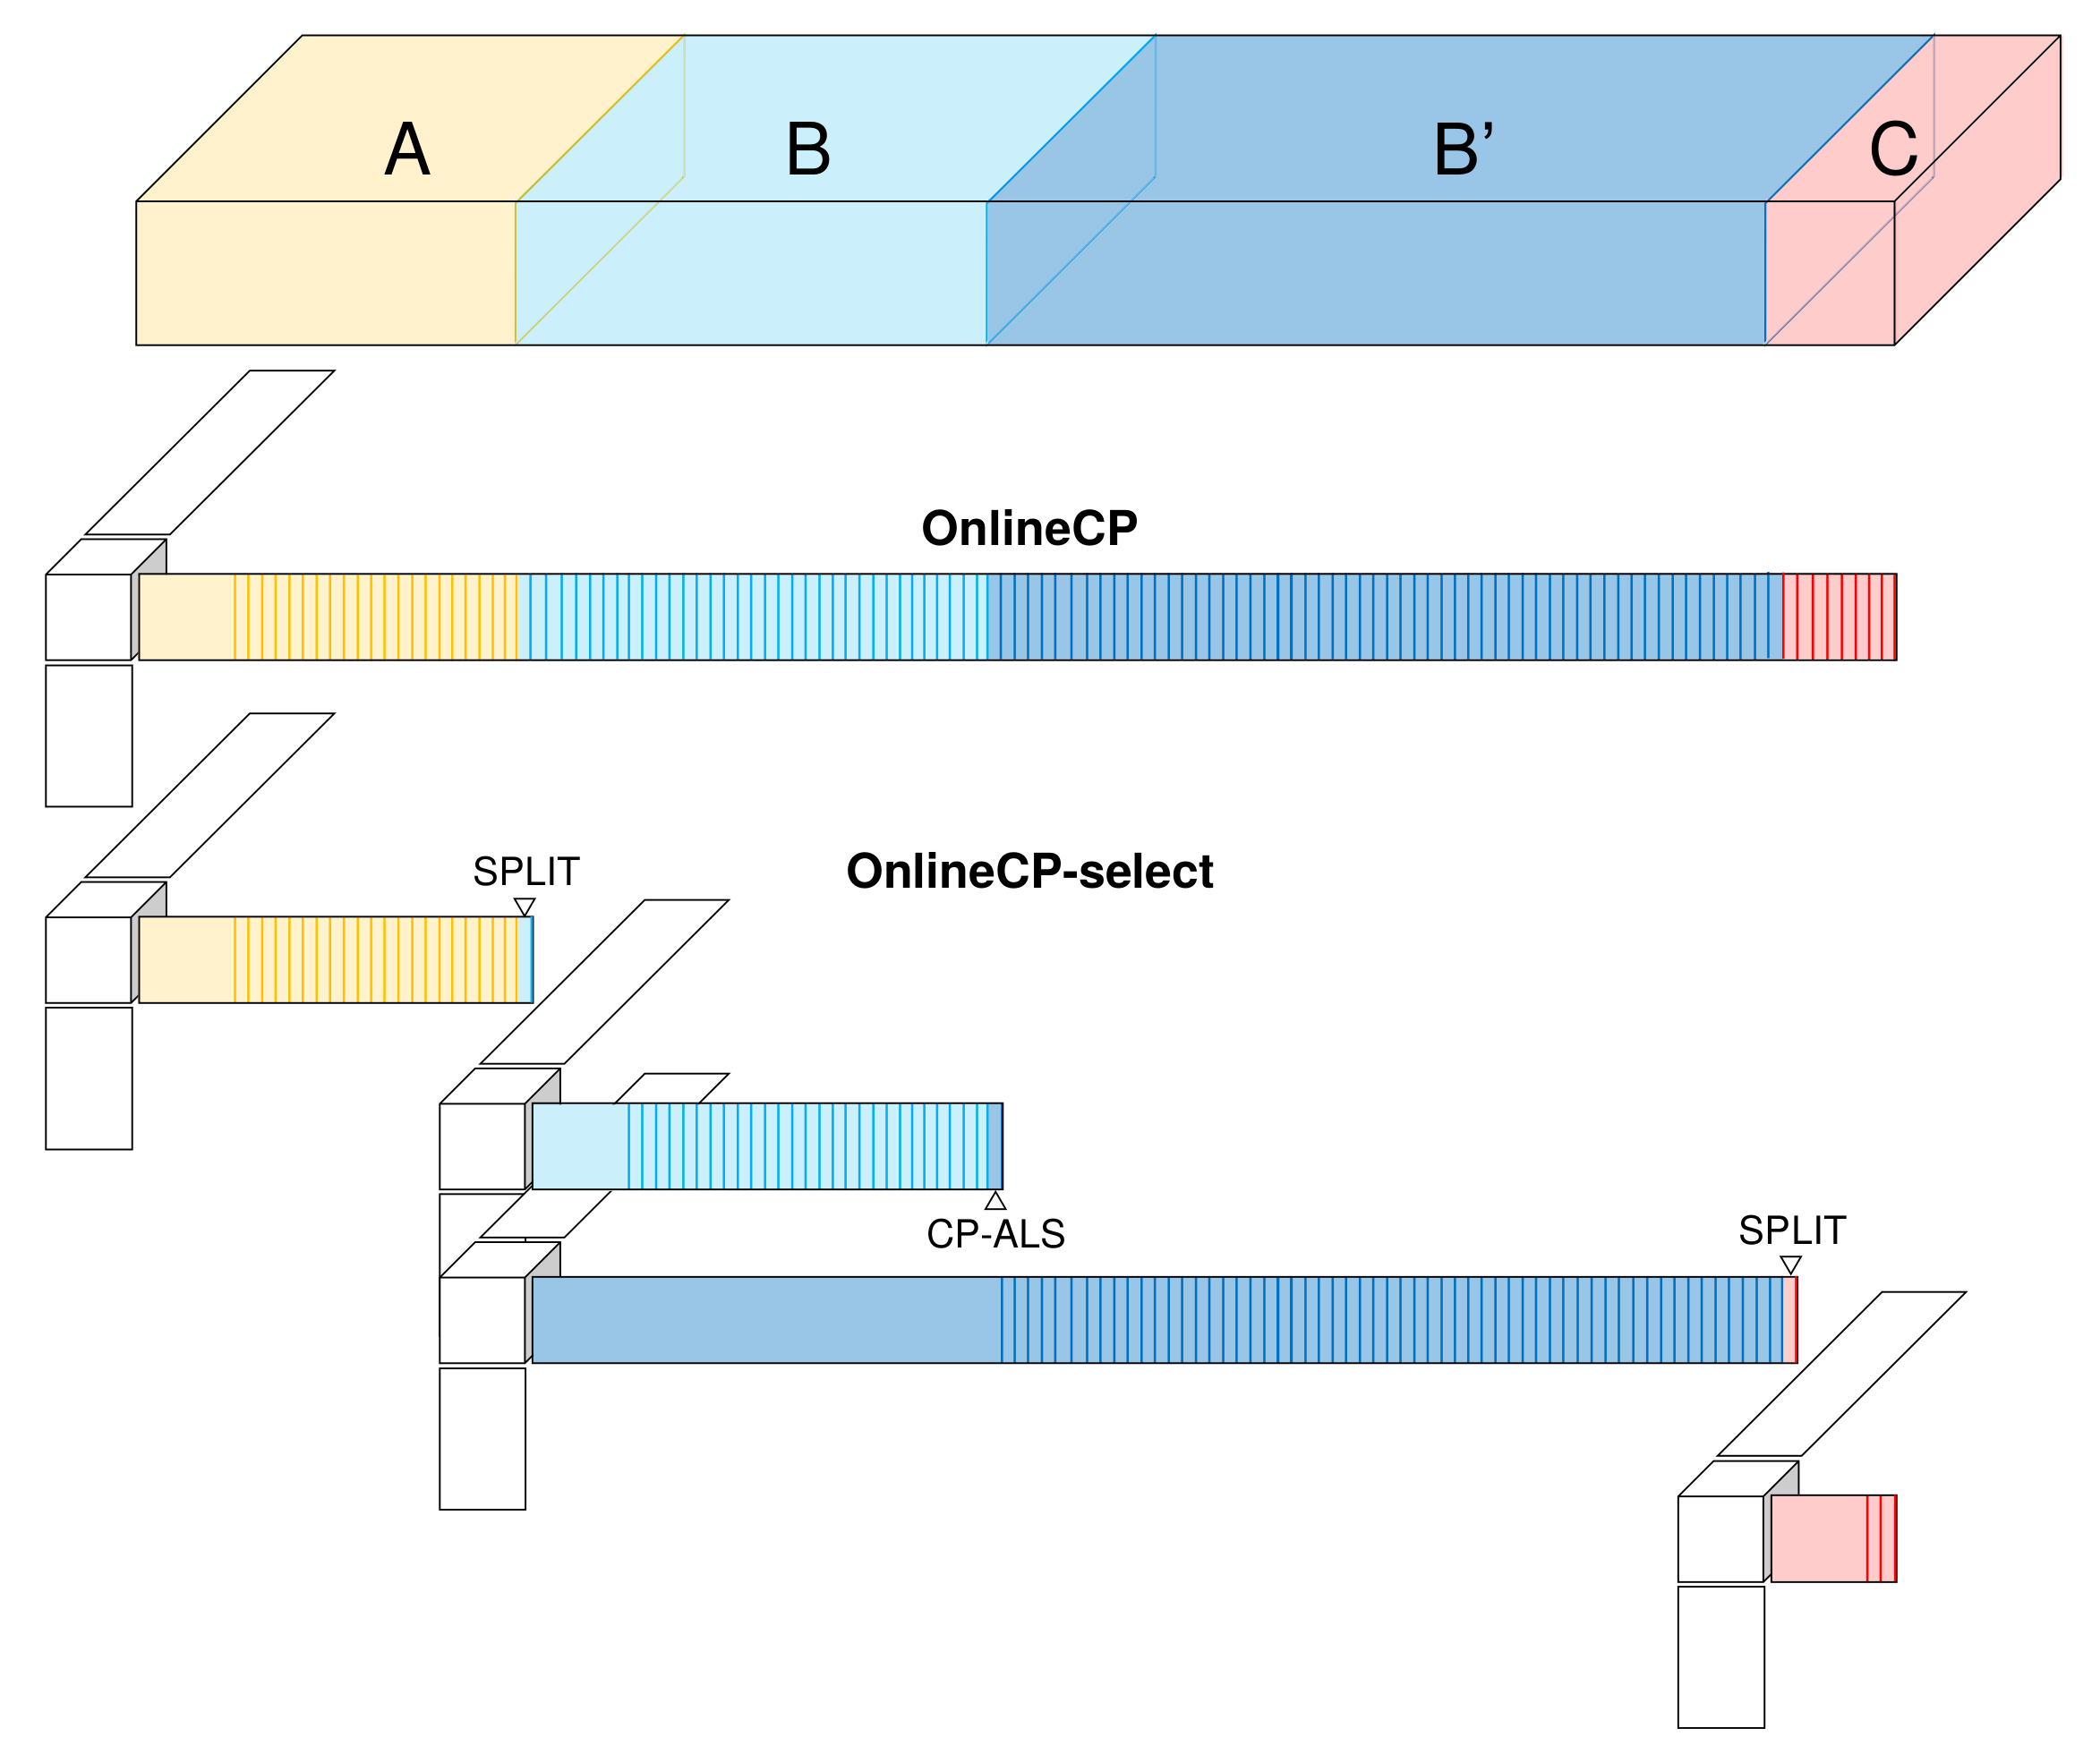
\includegraphics[width=0.9\textwidth]{FIG/OnlineCP-select.png}
\end{center}

\section{Experiments}
    \label{sec:experiments}
    

\subsection{Datasets}
For the demonstration, we will use a synthetic tensor and several real-world tensors. We've made stream of a tensor from starting point and split into parts with batch sizes. Here's our datasets and metadata to construct tensor streams.

\begin{table}[htb]
	\small
	\centering
	\begin{tabular}{ c | cccccc }
		\hline
		\textbf{Dataset} & \multicolumn{4}{c}{\textbf{Mode}} & \textbf{Start to Stream} & \textbf{Batch Sizes} \\
		\hline
 		Synthetic Data & 1 K & 10 & 20 & 30 & 5 & 5 * 199\\
 		Sample Video & 205 & 240 & 320 & 3 & 5 & 5 * 40\\
 		Stock & 3 K & 200 & 5 & & 10 & 10 * 299 \\
 		Sever Room CFD & 3 K & 3 & 3 & 34 & 10 & 10 * 299 \\
		\hline
	\end{tabular}
\end{table}

\subsubsection{\em Synthetic Data}
We've constructed synthetic data to manually make temporally changing points. This tensor has its size of $10*20*30*1000$ having the last mode as a temporal mode. The tensor was conducted by concatenation of theme tensor $T$ which is addition of three tensors $T_{main}$, $T_{theme}$ and $T_{noise}$. Each consisting tensor is 100x, 10x and 1x normal distributed randomized tensor respectively and those are used for making different and similar theme tensors.

\begin{table}[htb]
	\small
	\begin{tabular}{ c | cccccccccc }
 		\hline
 		Time Index & 1$\sim$100 & 101$\sim$200 & 201$\sim$250 & 251$\sim$500 & 501$\sim$600 & 601$\sim$700 & 701$\sim$750 & 751$\sim$800 & 801$\sim$950 & 951$\sim$1000 \\
 		\hline
 		Theme & $A$ & $A'$ & $B$ & $B'$ & $B''$ & $C$ & $D$ & $E$ & $E'$ & $E''$ \\
 		\hline
	\end{tabular}
\end{table}

\subsubsection{\em Sample Video}


\subsubsection{\em Stock}
KOSPI200

\subsubsection{\em Server Room CFD}
Temperature was measured in a server room equipped with two heterogeneously occupied racks and one roof-mounted cooling device by 34 probes. 3 servers power usage scenarios and also 3 air conditioning temperature scenarios were performed.

\newpage
\subsection{Experimental Results}
For each dataset, decomposition rank and number of iterations may affect performance of decomposition.
Triggering condition for split and refinement process depends on upper and lower limit of z-score, ${ul}$ and ${ll}$.

\begin{table}[htb]
	\small
	\centering
	\begin{tabular}{ c | cccc }
		\hline
		\textbf{Dataset} & \textbf{Rank} & \textbf{\# of Iterations} & \textbf{${ul}$} & \textbf{${ll}$} \\
		\hline
 		Synthetic Data & 10 & 1 & 1 & 0.5 \\
 		Sample Video & 20 & 1 & 5 & 3 \\
 		Stock & 5 & 5 & 5 & 3 \\
 		Sever Room CFD & 5 & 5 & 3 & 2 \\
		\hline
	\end{tabular}
\end{table}

\subsubsection{\em Sample Video}
\begin{center}
	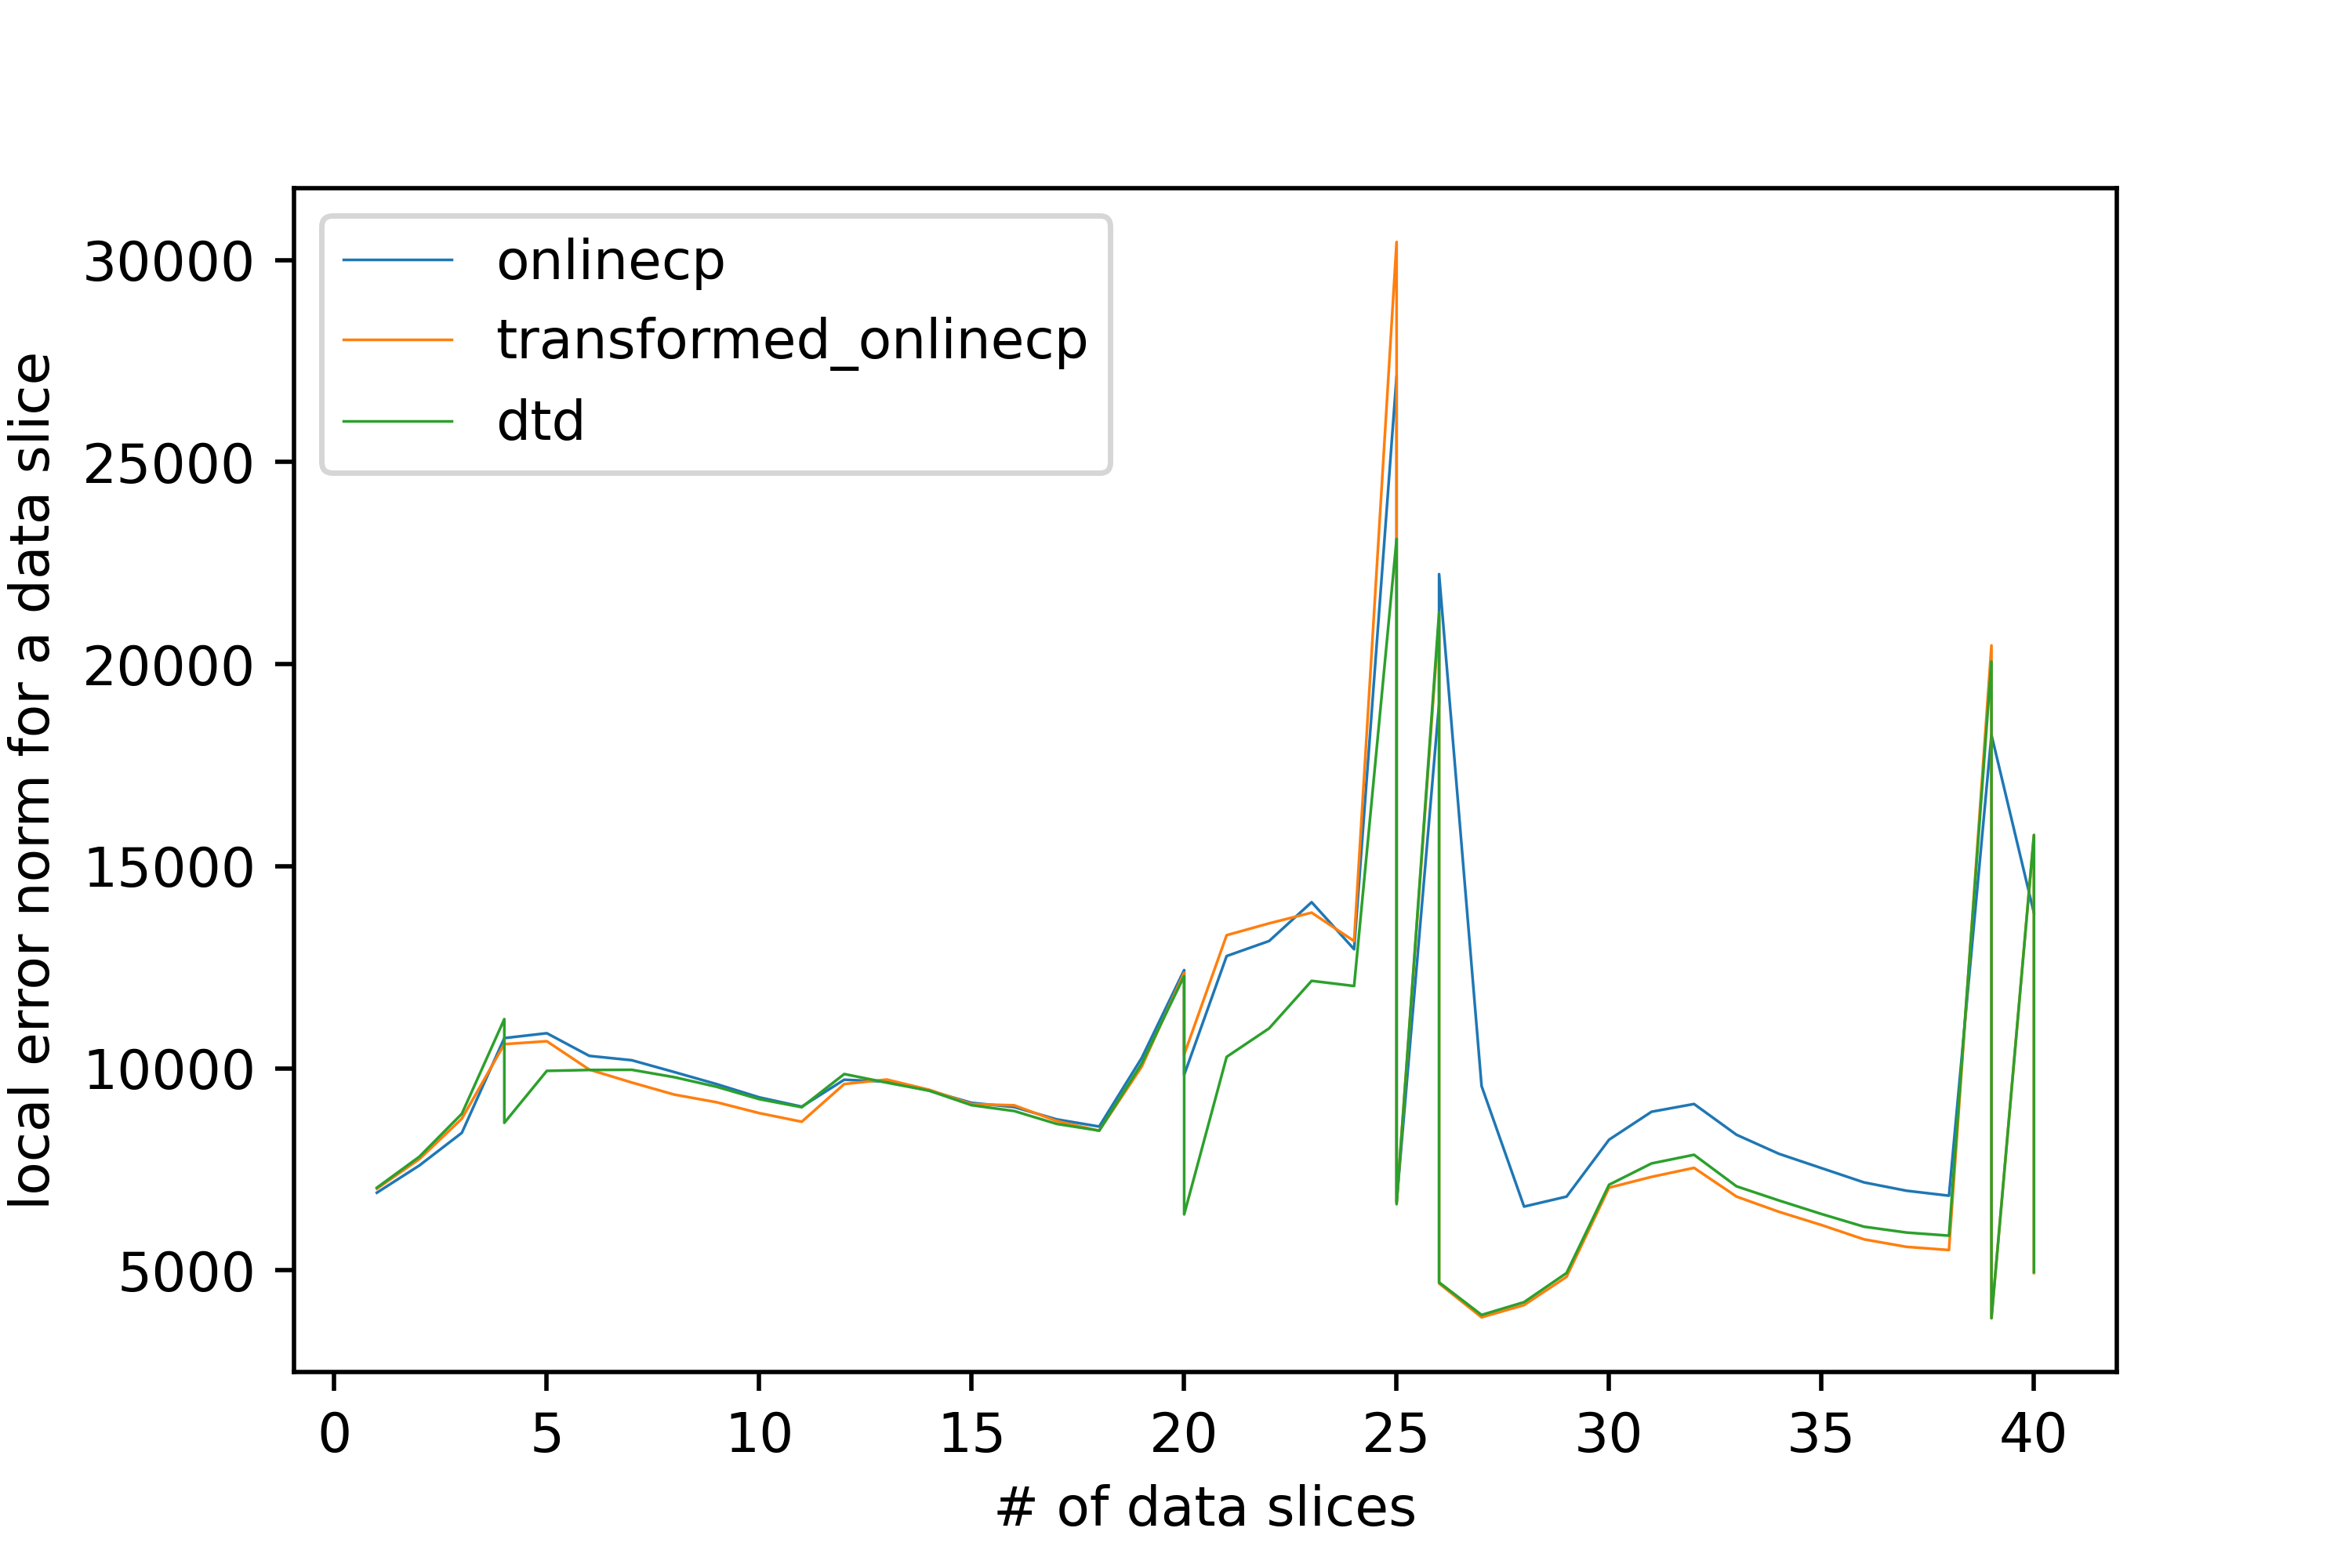
\includegraphics[width=0.49\textwidth]{FIG/sample_video_error_norm.png}
	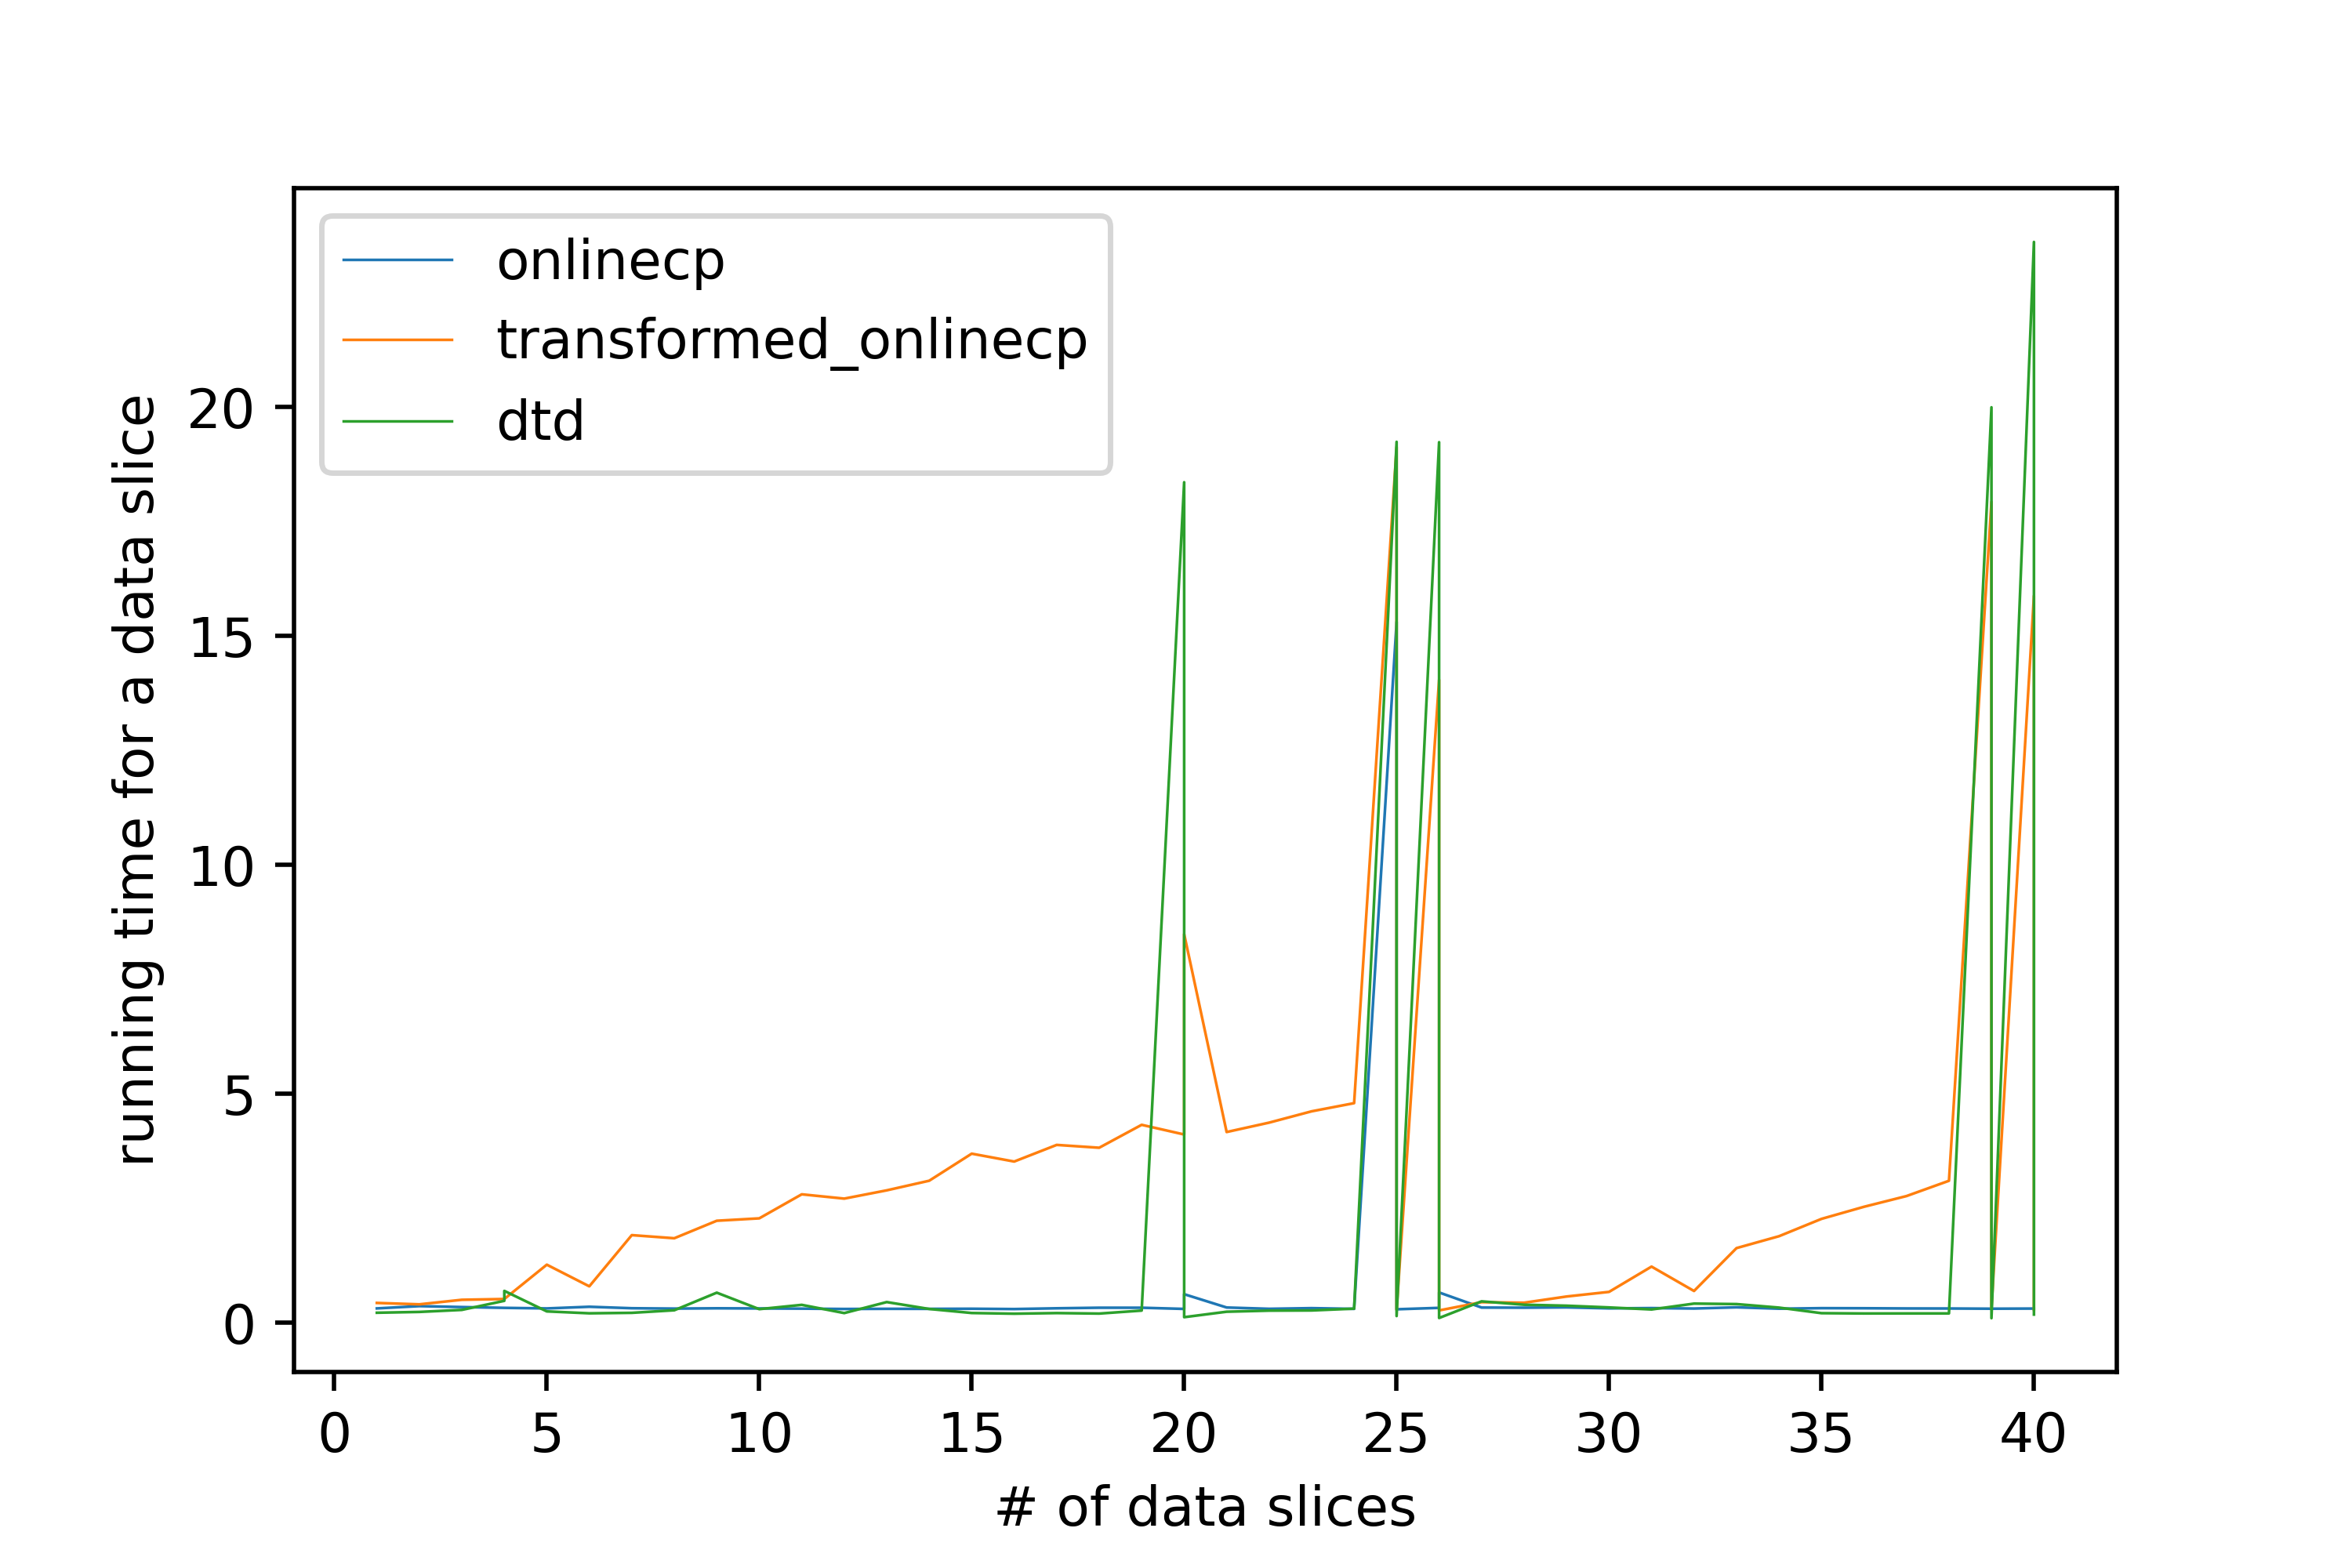
\includegraphics[width=0.49\textwidth]{FIG/sample_video_running_time.png}
\end{center}


\subsubsection{\em Stock}
\begin{center}
	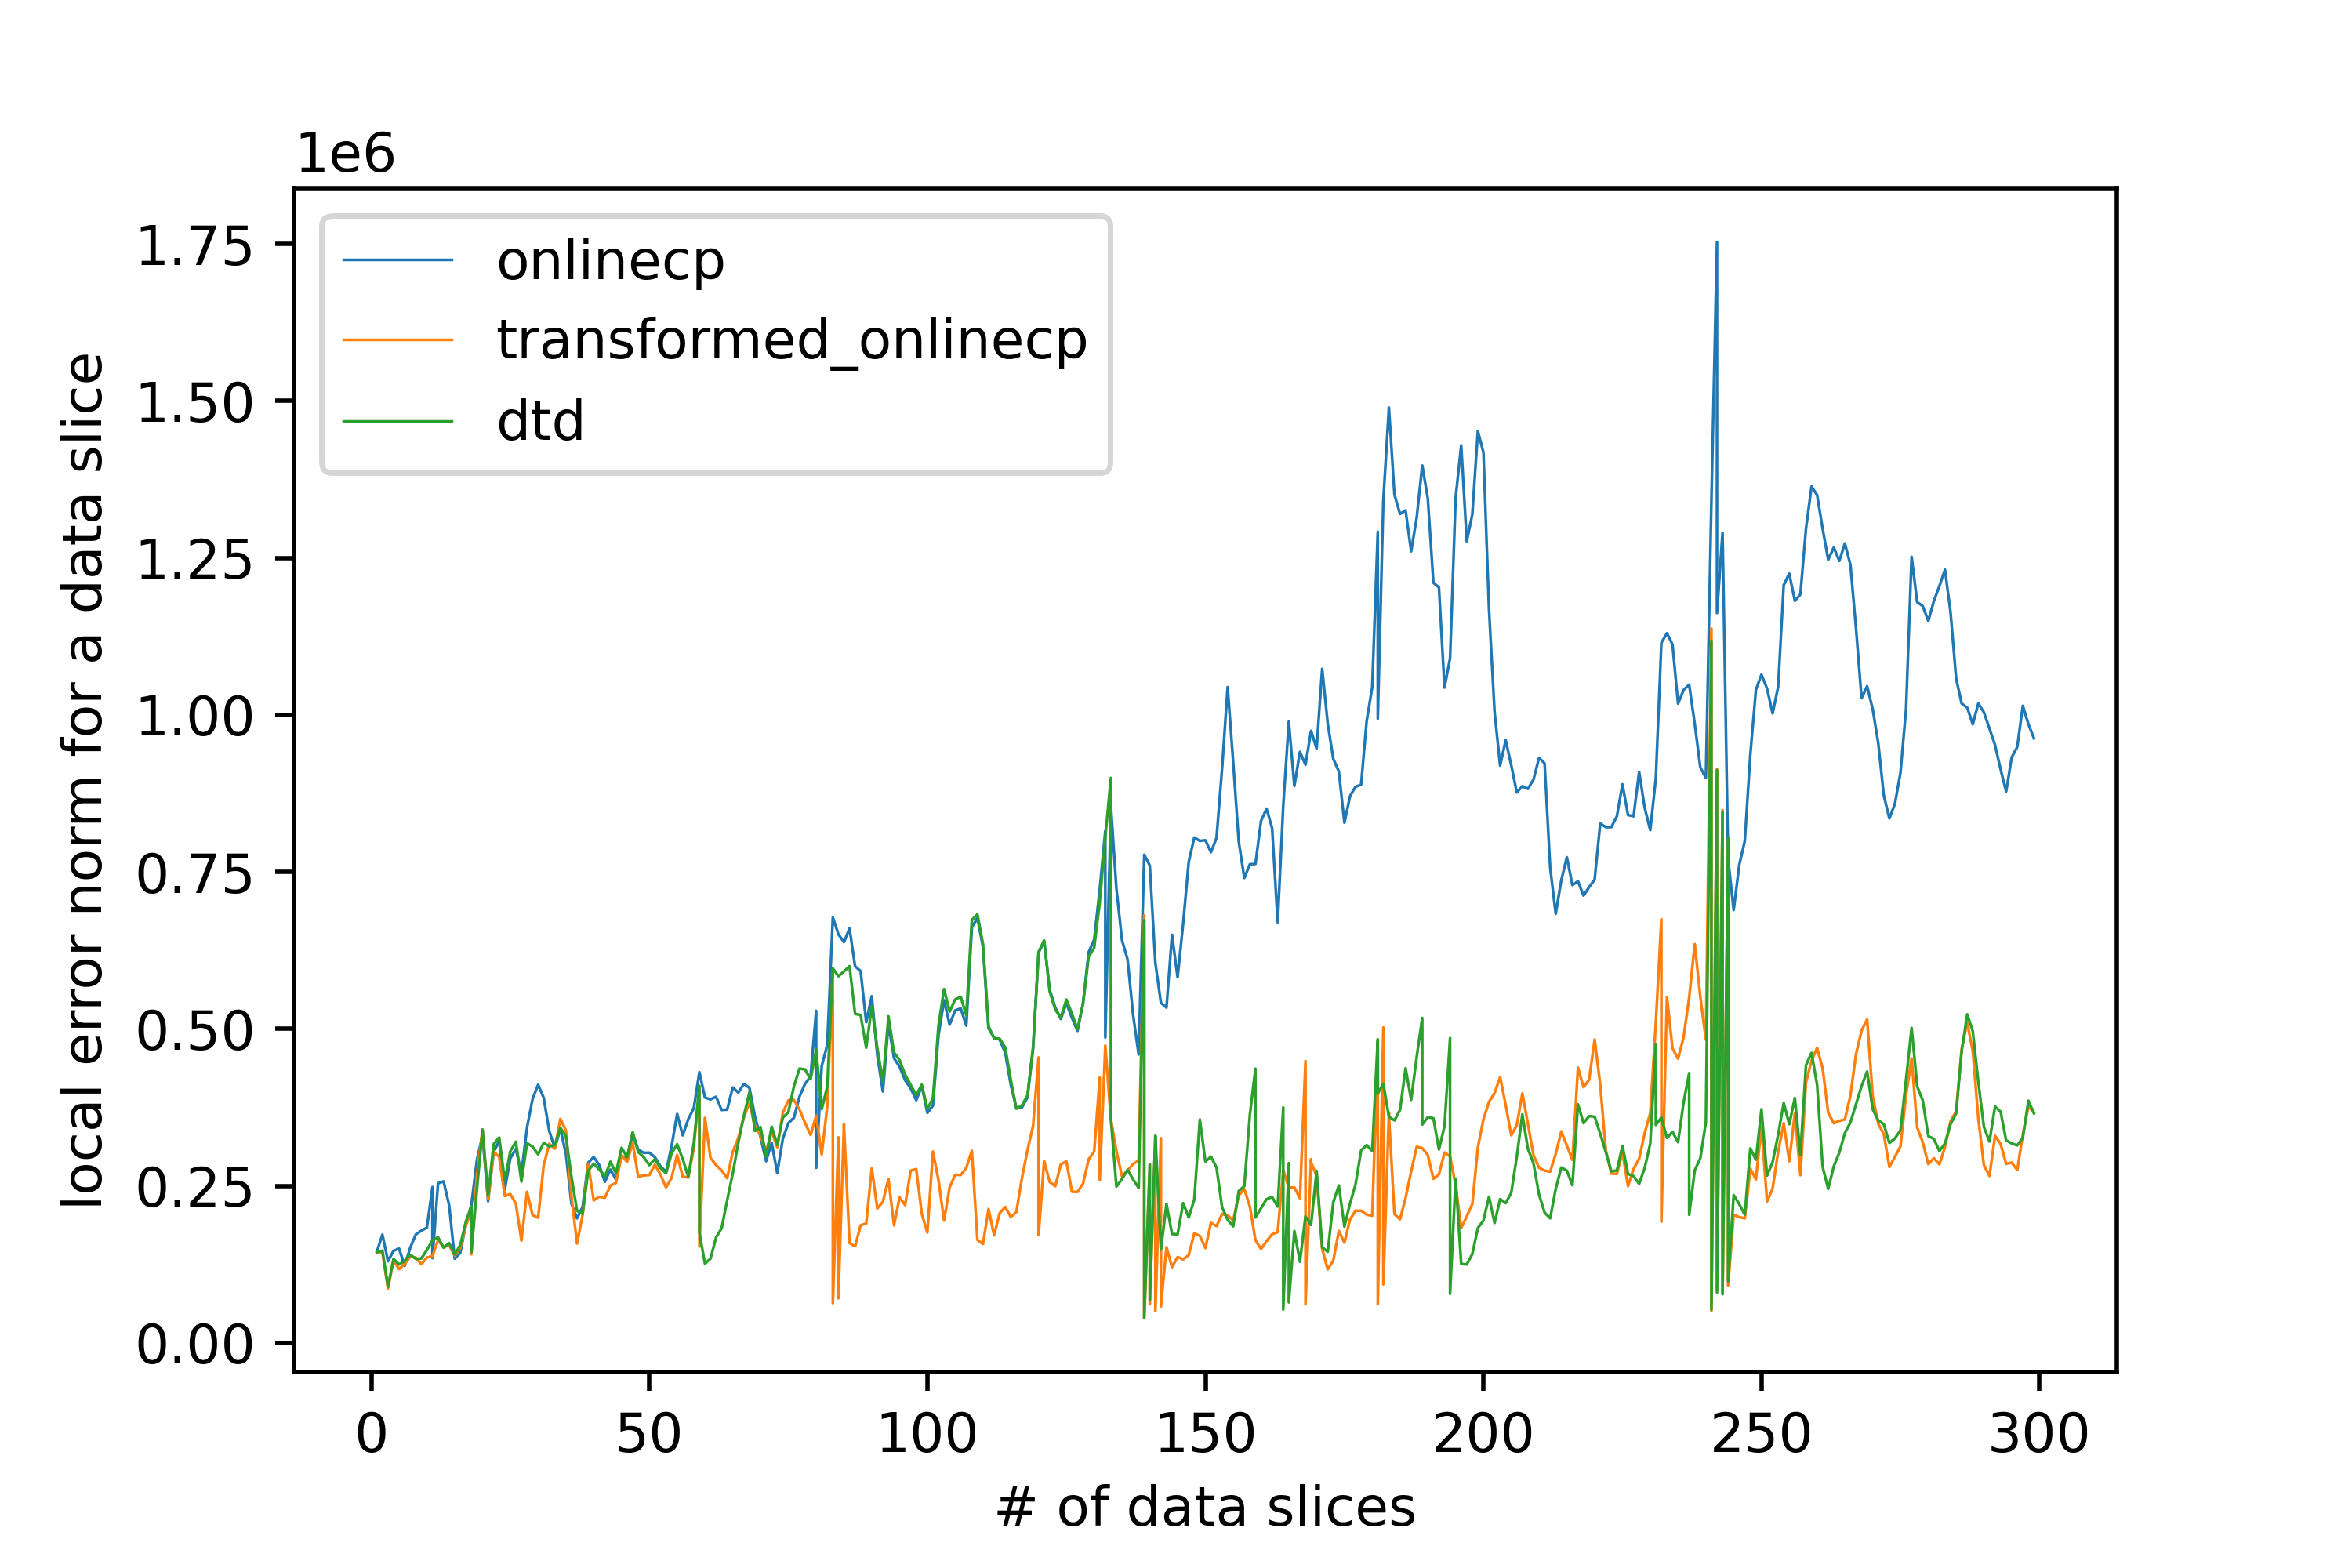
\includegraphics[width=0.49\textwidth]{FIG/stock_error_norm.png}
	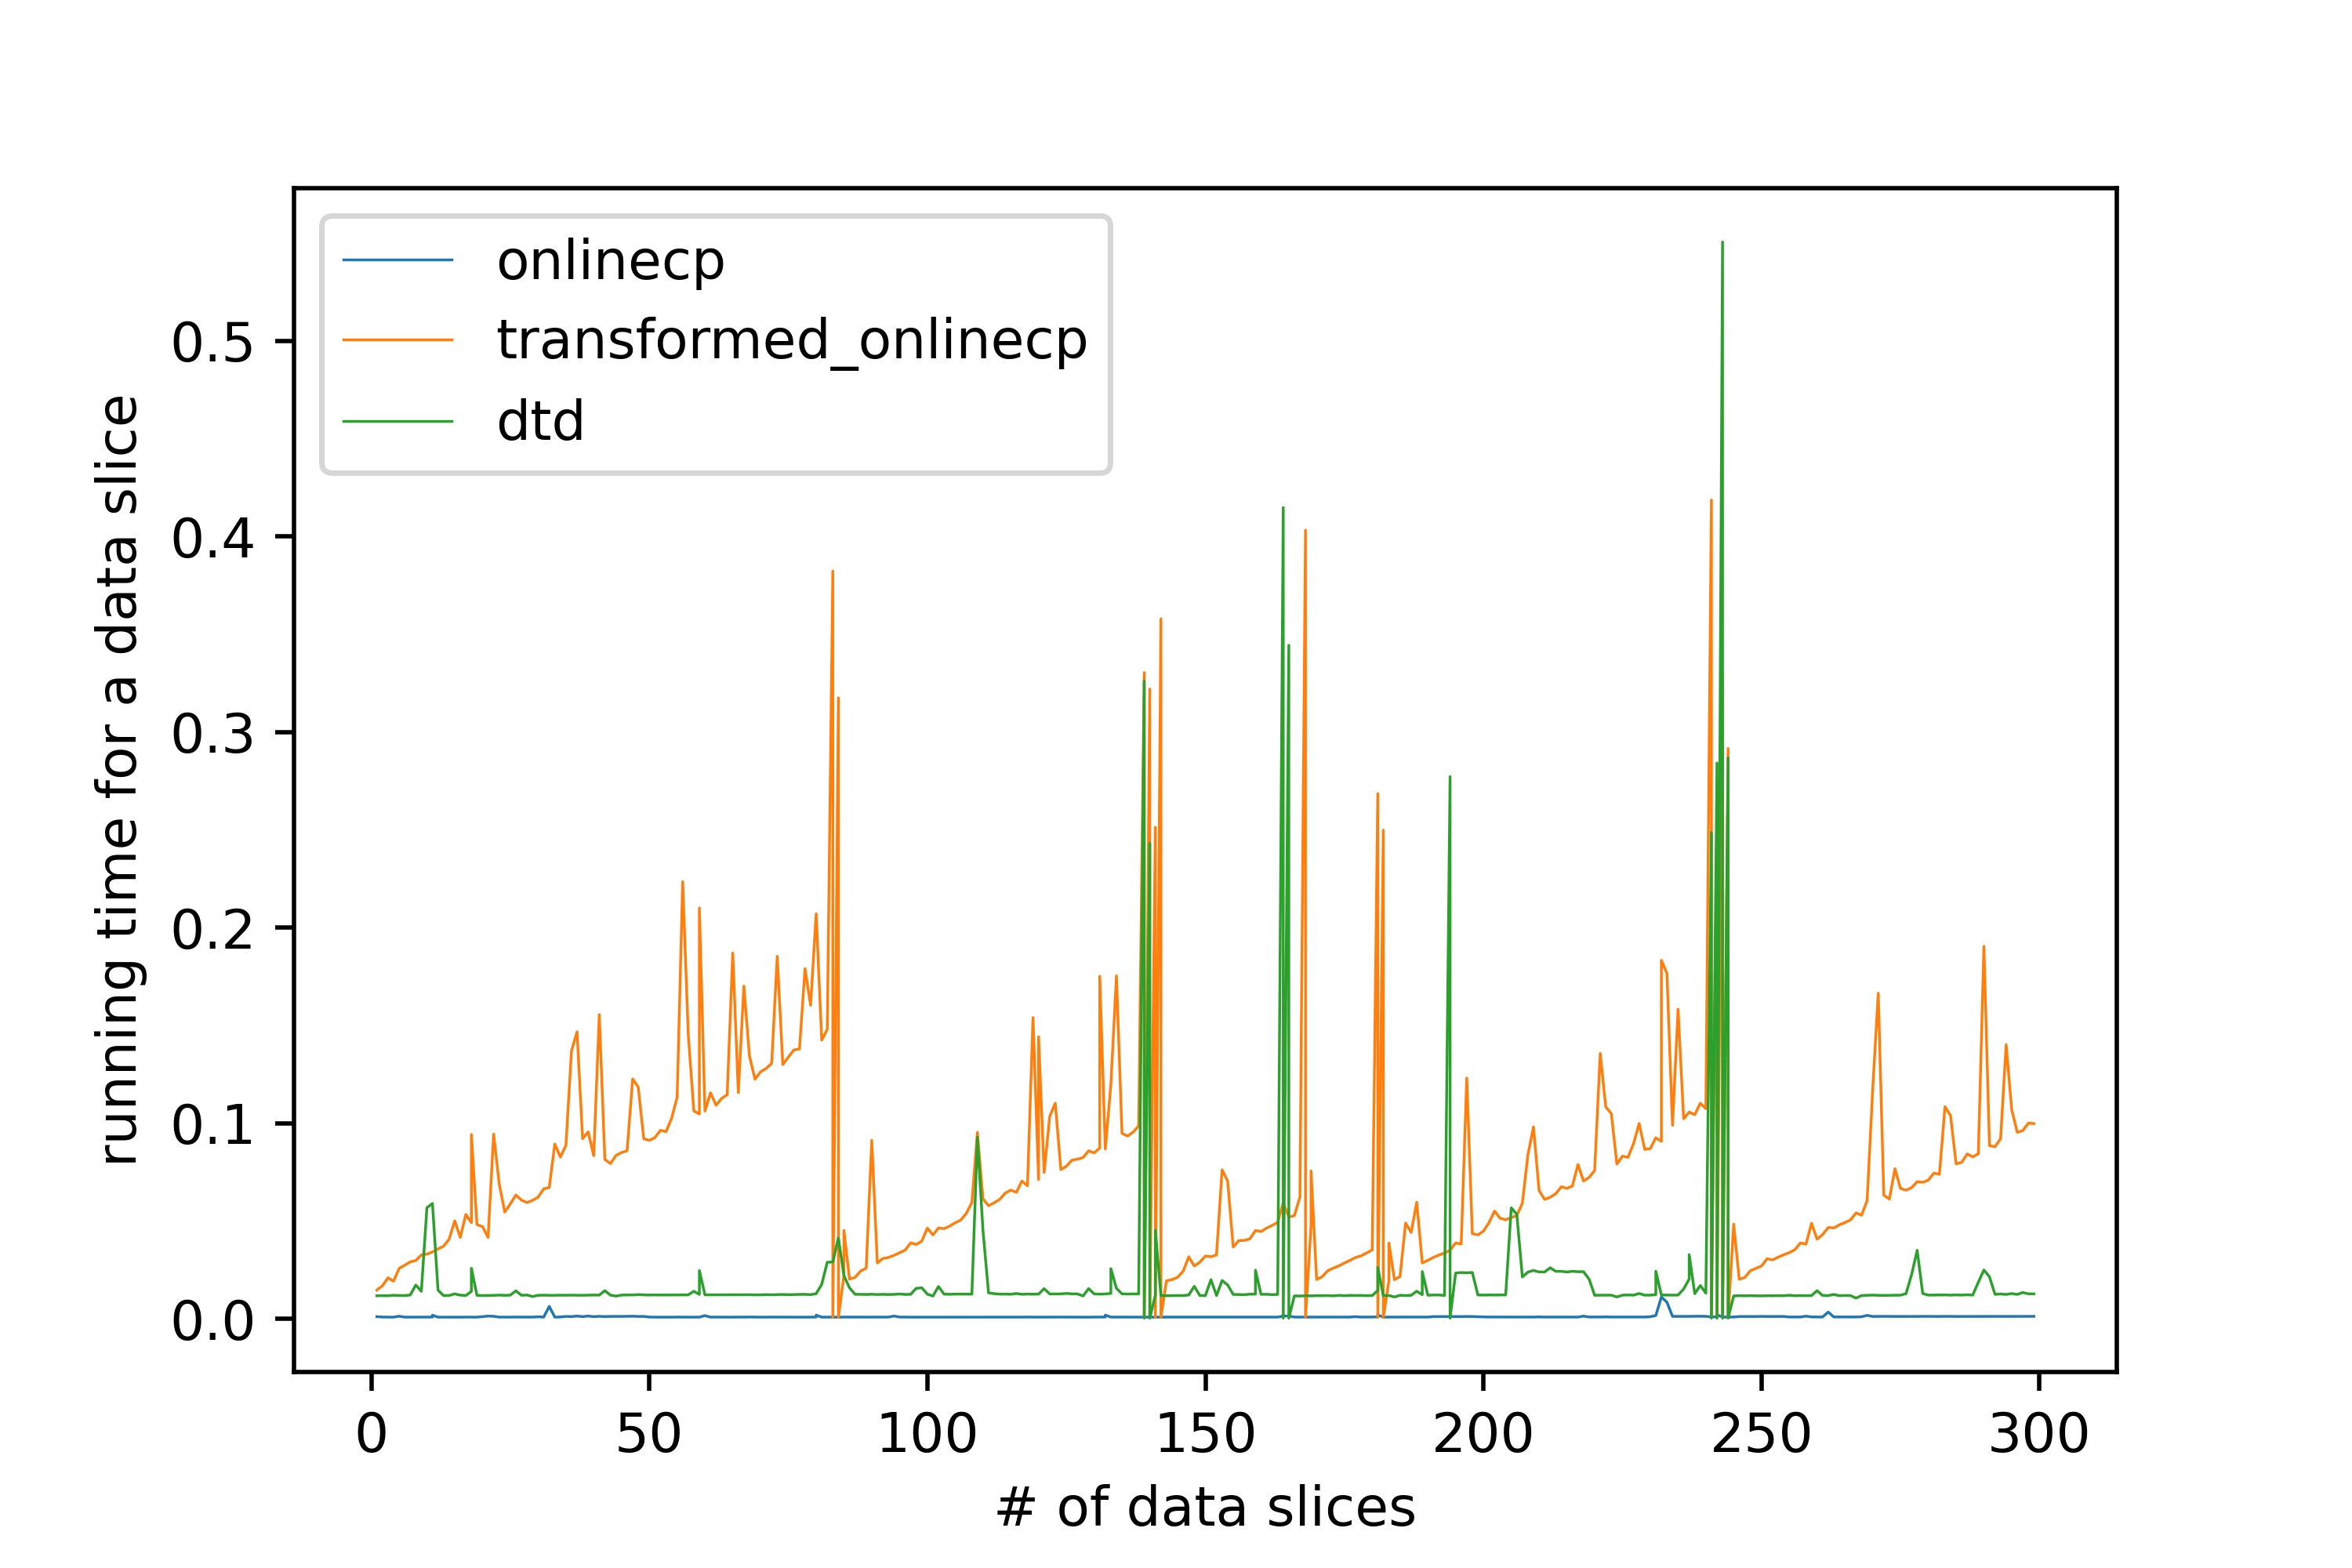
\includegraphics[width=0.49\textwidth]{FIG/stock_running_time.png}
\end{center}

    
\section{Related Works}
    \label{sec:related}
    Put related works here.    

\section{Conclusions}
    \label{sec:conclusions}
    The proposed method {\em someMETHOD}
has the following advantages:
\bit
\item it gives better classification accuracy than all 10 competitors we tried
\item its accuracy is very close to the very best competitor
      in the {\em UCR Insect Classification Contest}.
\item it is scalable
\eit



\bibliography{BIB/other}
\bibliographystyle{plain}

\newpage
\appendix
\section{Appendix}

\subsection{Additional Stuff 1}
Put contents here.

\subsection{Additional Stuff 2}
Put contents here.


\end{document}
